\section{Introduction}

After achieving extraordinary establishment in various fields of Machine Learning using neural networks, scientists began to move interests into network compression and enhancement. Several worth-mentioning approaches which seek to create smaller model and cost-efficient are parameter pruning/sharing, model quantization, low-rank factorization, and knowledge distillation. A comprehensive overview of these approaches is outside of the scope of this survey, and the focus of this paper is solely about knowledge distillation, which has attracted much attention from the deep learning research community in recent years. 

Comparing to other compression methods, KD might be considered superior since it can squeeze down a network disregarding the structural difference between the teacher and student network. The original idea of KD was proposed in \cite{firstkdpaper}, where the author focused on transferring the information from a large model or an ensemble of models into a smaller model without significant performance loss. This work is later generalized and popularized by Hinton et al. \cite{hintonfirstkd}. In their work, they found out an astounding observation that it is simpler to train a smaller-scale network (classifier) using the soften predictions of another classifier as target value rather than the ground truth (one-hot) labels and later on called this procedure as \textit{distillation} (short for knowledge distillation). They also stated that these probabilities offer richer information than labels alone, and empirically help the student network learn better. Knowledge distillation field since then has been developed and applied in various forms, but the main characteristic of KD has remained the same: Teacher-Student framework, where the teacher model provides useful \textit{knowledge} to the student model to improve its learning performance.

Thanks to its effectiveness on neural network compression and acceleration, KD has been widely applied in different fields of artificial intelligence: visual/speech recognition, natural language processing (NLP). In visual recognition, KD was firstly applied on classification tasks \cite{hintonfirstkd,visualtask01,visualtask02,visualtask03,visualtask04} then later on expanded to other applications such as image segmentation \cite{segment01}, lane detection \cite{lanedetect01}, facial landmark detection \cite{facial01, facial02}. In other fields such as NLP, KD also proves its worth as being used to compress complex structures such as BERT \cite{nlp01, nlp02}. To briefly generalized, KD offers not only lightweight deep models, which allows deploying models to on-edge devices efficiently but recently also competitive performant ones.
\begin{figure*}[h!]
   \begin{center}
      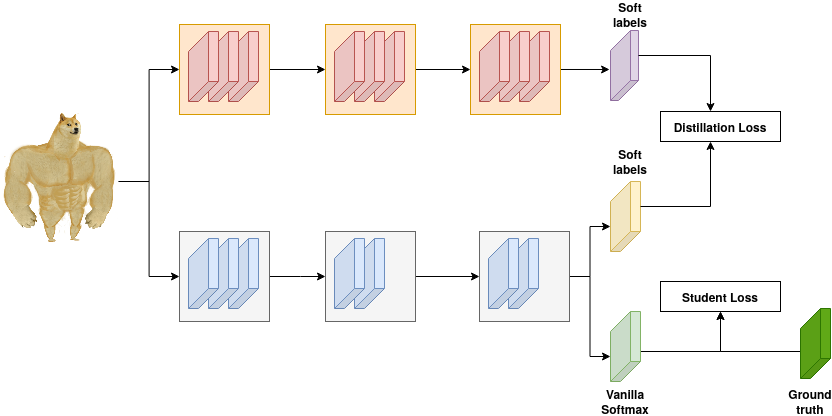
\includegraphics[width=0.8\linewidth]{assets/logits_based.png}
   \end{center}
      \caption{The typical architecture of logits-based knowledge distillation framework.}
   \label{fig:logits_base}
\end{figure*}

The main contributions of this paper consist of:
\begin{enumerate}
   \item Provide a comprehensive overview of Knowledge Distillation: problem definition, type of knowledge, a family of KD methods with deep learning.
   \item Investigate how the research community try to theoretically explain KD.
   \item Review several applicable regularization techniques used in distillation process.
\end{enumerate}
